\section{Technical Approach II --- Advanced Semantics \& Navigation}
\label{sec:adv}

Core semantics make one component correct; advanced semantics make a whole screen efficient to
navigate. They control how many focus stops exist, the order they are read in, and how nested actions
are reached, which create the difference between a automatically labelled UI and one that is fast to drive by
swipe or switch.

\subsection{Semantic merging}

By default every text node is its own focus stop. A podcast card with a cover, title, author, and
metadata therefore costs a TalkBack user 4--6 swipes to cross --- multiplied across a list of shows,
this is exhausting. \code{Modifier.semantics(mergeDescendants = true)} collapses a container's
children into one node whose announcement is the concatenation of its parts.

\begin{figure}[h]
	\centering
	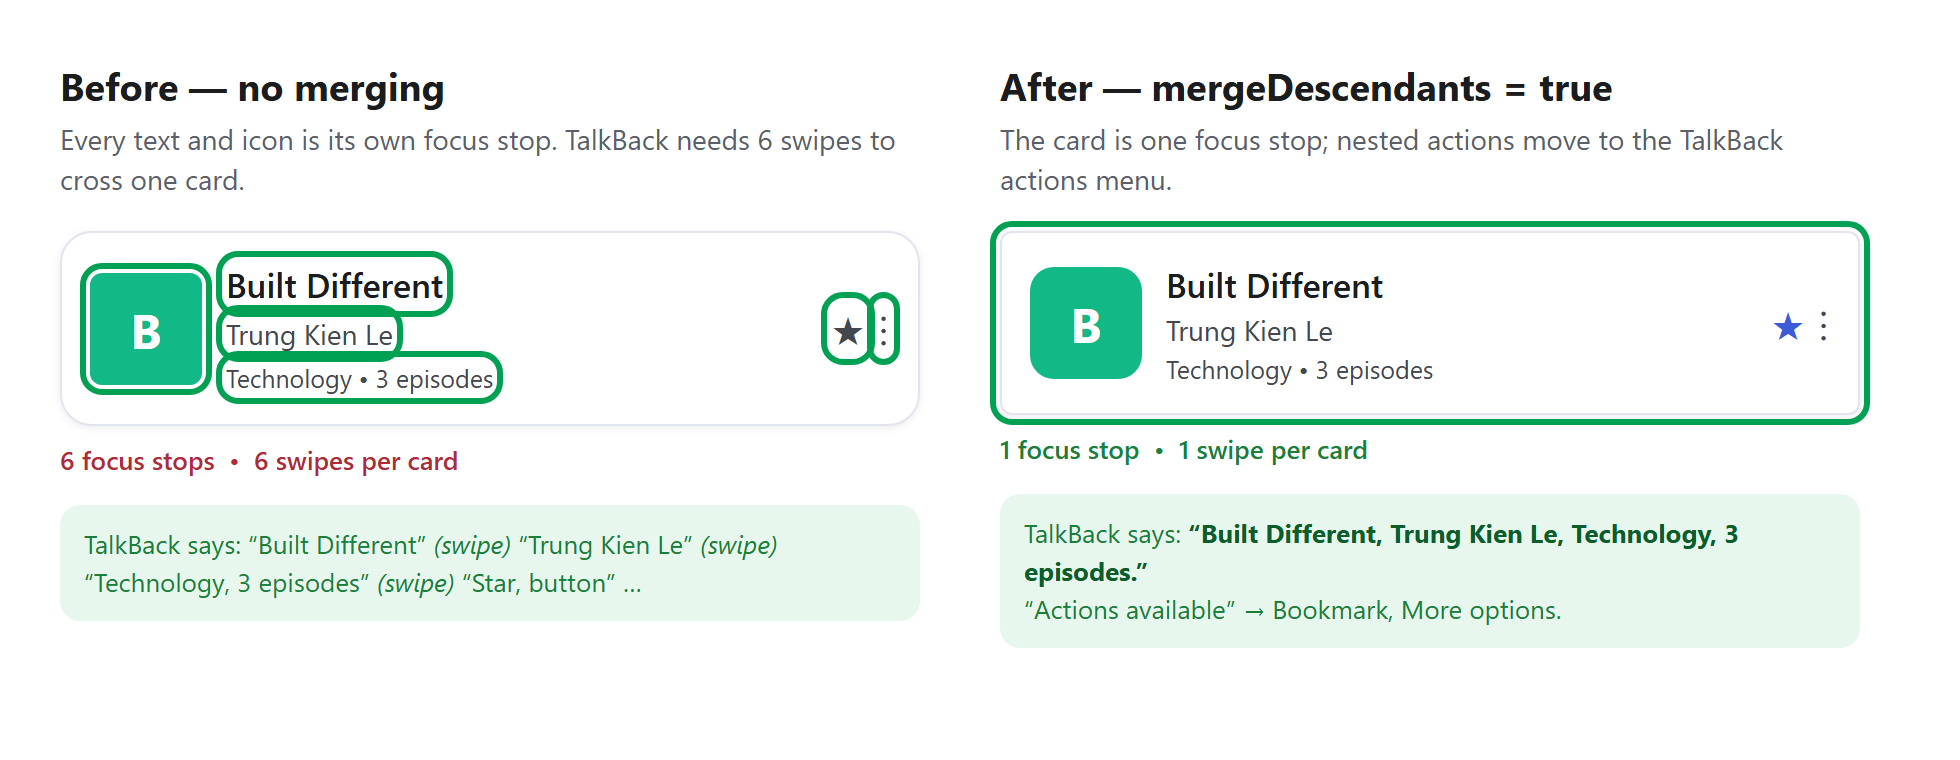
\includegraphics[width=\textwidth]{images/merge.png}
	\caption{The effect of \code{mergeDescendants = true} on a podcast card. Before (left): six separate
		focus stops, six swipes. After (right): one focus stop that TalkBack reads as a single sentence, with
		the nested bookmark/menu actions moved into the actions menu.}
	\label{fig:merge}
\end{figure}

\begin{lstlisting}[caption={\texttt{PodcastCard.kt} --- the card is one focus stop.},captionpos=b]
Card(
    onClick = onOpen,
    modifier = Modifier.semantics(mergeDescendants = true) {
        customActions = listOf(
            CustomAccessibilityAction(bookmarkLabel) { onToggleBookmark(latest); true }
        )
    }
) { /* cover + title + author + metadata + nested icon buttons */ }
\end{lstlisting}

There is a constraint on merging that a parent cannot merge a child that already merges itself. Interactive
components (\code{Button}, \code{Switch}, anything with \code{clickable}/\code{toggleable} modifiers) resist
merging so they remain independently operable. This is why the nested bookmark button needs
the next technique.

\subsection{Clearing and hiding with \texttt{clearAndSetSemantics} \& \texttt{hideFromAccessibility}}

Two modifiers prune the tree:

\begin{itemize}[leftmargin=1.4em]
	\item \code{clearAndSetSemantics \{\}} wipes a node's semantics (and its descendants') and lets us
	      redefine them  or leave them empty to remove the node from traversal entirely.
	\item \code{hideFromAccessibility()} (Compose~1.8+) hides a node from assistive services while
	      keeping it for UI tests. This is the modern alternative to setting
	      \code{contentDescription} to \code{null} on decorative elements.
\end{itemize}

In \code{CoverArt.kt} the coloured cover tile is decorative when a text title sits beside it, so we
hide it. In \code{EpisodeRow.kt} the three trailing icon buttons are cleared so they do not each
steal focus their actions are re-exposed on the row (next subsection).

\subsection{Custom accessibility actions}

Nested icon buttons are an anti-pattern for screen readers: they are tiny targets and they clutter
the swipe path (50 cards $\times$ 3 buttons = 150 extra swipes). The fix is to clear the
physical buttons and elevate their operations to \code{customActions} on the parent row, where
TalkBack surfaces them through its actions menu (``Actions available'').

\begin{lstlisting}[caption={\texttt{EpisodeRow.kt} --- nested actions promoted to the row's actions menu.},captionpos=b]
Row(
    modifier = Modifier.semantics(mergeDescendants = true) {
        customActions = listOf(
            CustomAccessibilityAction(playLabel)     { onPlay(); true },
            CustomAccessibilityAction(bookmarkLabel) { onToggleBookmark(); true },
            CustomAccessibilityAction(downloadLabel) { onToggleDownload(); true },
        )
    }
) {
    FilledIconButton(onClick = onPlay,
        modifier = Modifier.size(48.dp).clearAndSetSemantics {}) { /* icon */ }
    // ... title + metadata ...
    IconButton(onClick = onToggleBookmark,
        modifier = Modifier.minimumInteractiveComponentSize().clearAndSetSemantics {}) { /* icon */ }
}
\end{lstlisting}

A screen-reader user now hears the episode as one sentence, then opens ``Actions'' to Play, Bookmark,
or Download, while sighted users still tap the visible 48\,dp buttons directly.

\subsection{Traversal order}

Assistive tech normally reads in fixed order (top-to-bottom, then left-to-right), which breaks on non-linear
layouts. Two modifiers fix it: \code{isTraversalGroup = true} draws a boundary that must be read
completely before moving on, and \code{traversalIndex} (a \code{Float}, lowest first) reorders within
that boundary. A common pitfall is setting \code{traversalIndex} \emph{without} a group: because all
nodes default to \code{0f} globally, the element is compared against the whole screen and jumps to the
bottom. On the Discover screen we make the ``Continue listening'' banner read \emph{first} even though
it is not the top-most focusable item:

\begin{lstlisting}[caption={\texttt{HomeScreen.kt} --- resume banner announced first via a low traversal index.},captionpos=b]
LazyColumn(modifier = Modifier.semantics { isTraversalGroup = true }) {
    item {
        ContinueListeningBanner(
            modifier = Modifier.semantics { traversalIndex = -1f } // read before everything else
        )
    }
    // ... section header + podcast cards ...
}
\end{lstlisting}

\subsection{Decision matrix}

Table~\ref{tab:matrix} summarises when to reach for each advanced modifier.

\begin{table}[h]
	\centering
	\small
	\begin{tabularx}{\textwidth}{@{}l l Y@{}}
		\toprule
		\textbf{API}                       & \textbf{Applied to}         & \textbf{Use case / effect}                              \\
		\midrule
		\code{mergeDescendants = true}     & Container (Row/Column/Card) & Fuse fragmented text into one focus stop.               \\
		\code{clearAndSetSemantics \{\}}   & Custom or nested nodes      & Erase raw semantics; redefine or remove from traversal. \\
		\code{hideFromAccessibility()}     & Decorative elements         & Hide from TalkBack, keep for UI tests.                  \\
		\code{isTraversalGroup = true}     & Layout container            & Force children to be read as a bounded block.           \\
		\code{traversalIndex = Xf}         & Child of a traversal group  & Reorder reading (lowest value read first).              \\
		\code{customActions = listOf(...)} & Parent list item / card     & Move nested actions into the TalkBack menu.             \\
		\bottomrule
	\end{tabularx}
	\caption{Choosing an advanced semantics API by structural need.}
	\label{tab:matrix}
\end{table}
